\documentclass[a4paper, 11pt, oneside]{article}

\usepackage[utf8]{inputenc}
\usepackage[T1]{fontenc}
\usepackage[english]{babel}
\usepackage{array}
\usepackage{shortvrb}
\usepackage{listings}
\usepackage[fleqn]{amsmath}
\usepackage{amsfonts}
\usepackage{fullpage}
\usepackage{enumerate}
\usepackage{graphicx}
\usepackage{alltt}
\usepackage{indentfirst}
\usepackage{eurosym}
\usepackage{titlesec, blindtext, color}
\usepackage[table,xcdraw,dvipsnames]{xcolor}
\usepackage[unicode]{hyperref}
\usepackage{url}
\usepackage{float}
\usepackage{subcaption}
\usepackage[skip=1ex]{caption}

\definecolor{brightpink}{rgb}{1.0, 0.0, 0.5}

\usepackage{titling}
\renewcommand\maketitlehooka{\null\mbox{}\vfill}
\renewcommand\maketitlehookd{\vfill\null}

\newcommand{\ClassName}{ELEN-0060: Information and Coding Theory}
\newcommand{\ProjectName}{Project 2 - Source coding, data compression and \\ channel coding}
\newcommand{\AcademicYear}{2021 - 2022}

%%%% First page settings %%%%

\title{\ClassName\\\vspace*{0.8cm}\ProjectName\vspace{1cm}}
\author{Maxime Goffart \\180521 \and Olivier Joris\\182113}
\date{\vspace{1cm}Academic year \AcademicYear}

\begin{document}

%%% First page %%%
\begin{titlingpage}
{\let\newpage\relax\maketitle}
\end{titlingpage}

\thispagestyle{empty}
\newpage

%%%%%%%%%%%%%%%%%%%%%%%%%%%%%%%%%%%%%%%%%%

%%% Table of contents %%%
%\tableofcontents
%\newpage

%%%%%%%%%%%%%%%%%%%%%%%%%%%%%%%%%%%%%%%%%%

% CONTENT %



%%%%%%%%%%%%%%%%%%%%%%%%%%%%%%%%%%%%%%%%%%
\section{Channel coding}

\subsection{Question 16}
\paragraph{}In order to implement a function to read and display the given image, we used the methods \texttt{imread} and \texttt{imshow} provided by OpenCV.

%%%%%

\subsection{Question 17}
\paragraph{}To encode the image signal, we used a fixed-length binary code of 8 bits. We have chosen 8 bits because there are 256 (from 0 to 255) possible values, so we need $\lceil log_2(256) \rceil =8$.\\
The code is the binary representation of the grayscale value of each pixel.

%%%%%

\subsection{Question 18}
\paragraph{}By simulating the channel effect on the binary signal of the image, we get the following image:
\begin{figure}[H]
    \centering
    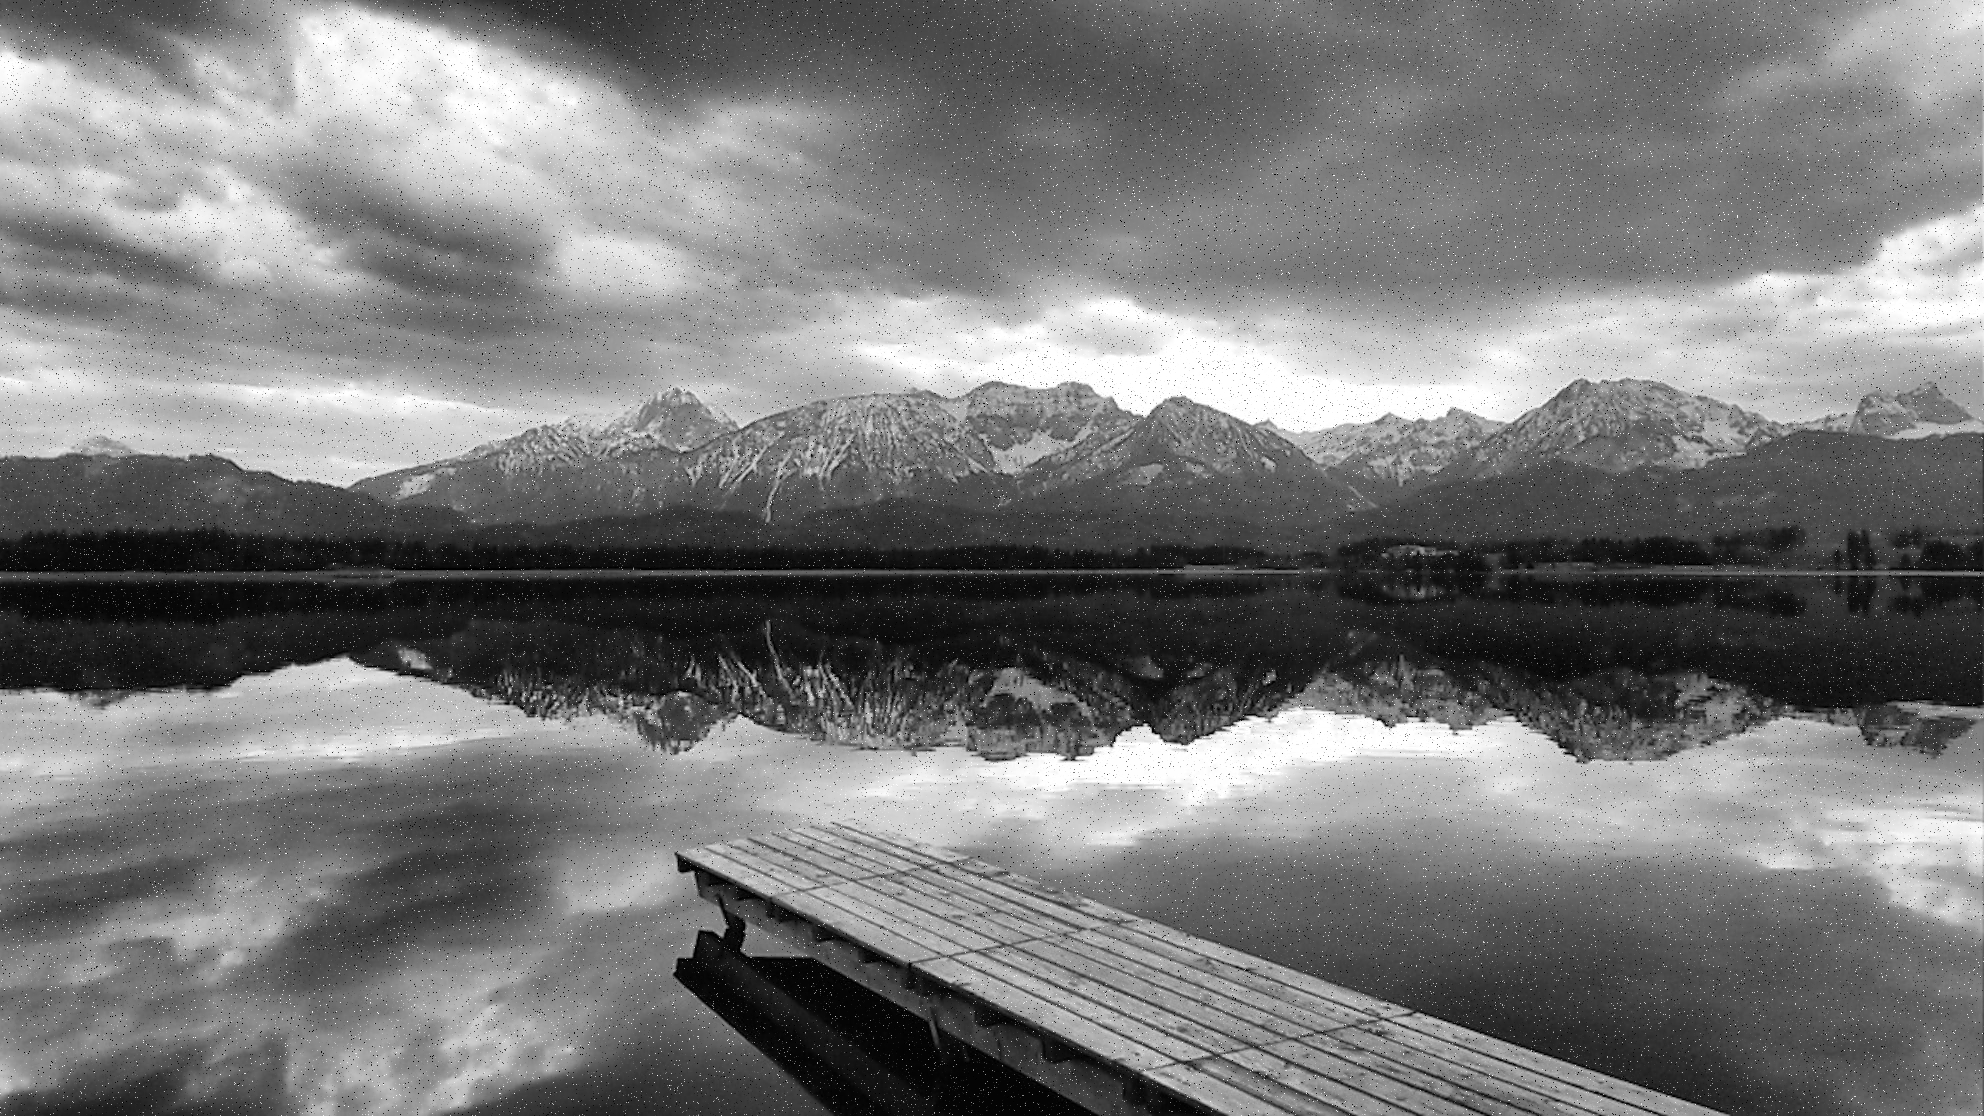
\includegraphics[scale=0.2]{q18.png}
    \caption{Image after simulating the channel effect}
\end{figure}
As we can see in the picture, after simulating the channel effect, there are a lot of small dots that are pixels with different grayscale values
compared to there very close neighbors.\\
This is due to the fact that we are simulating a potential loss bit by bit and we are not using any sort of redundancy.
Thus, if one of the most significant bits is modified, it completely changes the grayscale value for the pixel.

%%%%%%%%%%%%%%%%%%%%%%%%%%%%%%%%%%%%%%%%%%

\end{document}